\ylDisplay{Türistor} % Ülesande nimi
{Jaan Toots} % Autor
{lõppvoor} % Voor
{2015} % Aasta
{G 10} % Ülesande nr.
{10} % Raskustase
{
% Teema: Elektriahelad
\ifStatement
\begin{wrapfigure}{r}{0.48\textwidth}
\begin{circuitikz} \draw

(0,2) to[resistor=$R$] (2,2)
      to[Do,l=$T_1$, *-*] (2,0) -- (0,0)
      to[battery1,l=$U$] (0,2)
(2,2) to[switch] (4,2)
      to[Do,l=$T_2$] (4,0) -- (2,0)
;
\end{circuitikz}
\end{wrapfigure}
Türistori (dioodisarnase elemendi) volt-amper karakteristik on juuresoleval graafikul. Kaks sellist türistori on ühendatud pingeallika ja takistiga kõrvalolevasse skeemi. Takistus $R = \SI{2}{\kilo\ohm}$.\\
{\bf a}) Alguses on lüliti avatud. Pingeallika pinget suurendatakse lineaarselt $t=\SI{42}{\second}$ jooksul väärtuselt $U_0=\SI{0}{\volt}$ kuni väärtuseni $U_a = \SI{42}{\volt}$. Skitseerige ahelat läbiva voolutugevuse $I(t)$ sõltuvus ajast. Milline on voolutugevuse lõppväärtus $I_a$?\\
{\bf b}) Leidke lõppvoolutugevused mõlemas türistoris, kui lüliti suletakse ilma ahelale rakendatud pinget $U_a$ muutmata.

\begin{figure}[h]
\begin{center}
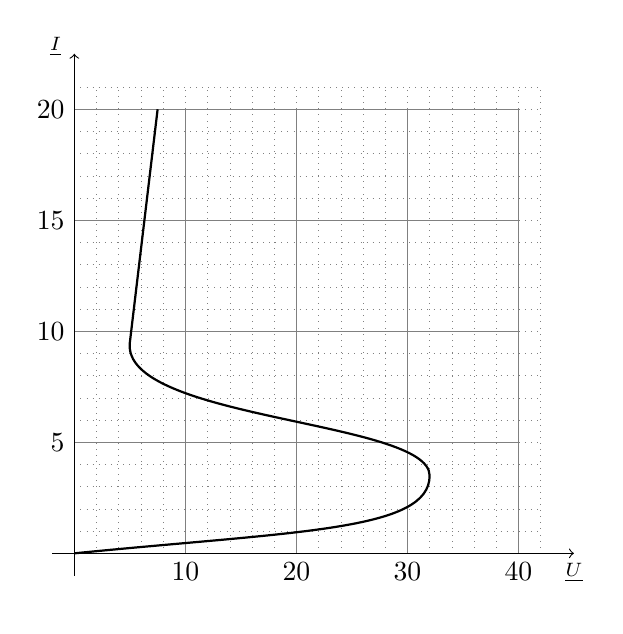
\begin{tikzpicture}[scale=1.41,
axes/.style=]

\draw[step=0.2, gray, dotted, very thin] (0,0) grid (4.2,4.2);
\draw[step=1, gray, very thin] (0,0) grid (4,4);

\begin{scope}[axes]
    \draw[->] (-0.2,0) -- (4.5,0) node[right, below] {$\frac{U}{\si{\volt}}$} coordinate(x axis);
    \draw[->] (0,-0.2) -- (0,4.5) node[above, left] {$\frac{I}{\si{\milli\ampere}}$} coordinate(y axis);

    \foreach \x/\xtext in {1/10, 2/20, 3/30, 4/40}
    \draw (\x,0) node[below] {$\xtext$};
    
    \foreach \y/\ytext in {1/5, 2/10, 3/15, 4/20}
    \draw (0,\y) node[left] {$\ytext$};
\end{scope}

\draw[thick] (0,0) .. controls (2,0.2) and (3.2,0.2) .. (3.2,0.7) .. controls (3.2,1.2) and (5/12,1.2) .. (0.5,1.9) -- (0.75,4);

\end{tikzpicture}

\end{center}
\end{figure}
\fi


\ifHint
Kirchhoffi esimese seaduse põhjal peab suvalise pinge ja voolutugevuse korral kehtima $V = U - IR$, kus $V$ on pinge türistoril. Kandes vastava funktsiooni volt-amperkarakteristikule on näha, et mingi pinge $U$ korral on $I$ ja $V$ jaoks kuni kolm lahendit, kusjuures negatiivse tõusuga punkt ei ole stabiilne, kuna vastaks negatiivsele takistusele. Antud informatsiooniga on võimalik määrata, kuidas türistorit läbiv vool muutub pingeallika pinge tõstmisel.
\fi


\ifSolution
\begin{figure}[h]
\begin{center}
\begin{tikzpicture}[scale=1.4,
axes/.style=]

%\draw[step=0.2, gray, dotted, very thin] (0,0) grid (4,4);
\draw[step=1, gray, ultra thin] (0,0) grid (4,4);

\begin{scope}[axes]
    \draw[->] (-0.2,0) -- (4.5,0) node[below] {$\frac{V_1}{\si{\volt}}$} coordinate(x axis);
    \draw[->] (0,-0.2) -- (0,4.5) node[left] {$\frac{I}{\si{\milli\ampere}}$} coordinate(y axis);

    \foreach \x/\xtext in {1/10, 2/20, 3/30, 4/40}
    \draw (\x,0) node[below] {$\xtext$};
    
    \foreach \y/\ytext in {1/5, 2/10, 3/15, 4/20}
    \draw (0,\y) node[left] {$\ytext$};
\end{scope}

\draw [thick, name path=func] (0,0) .. controls (2,0.2) and (3.2,0.2) .. (3.2,0.7) .. controls (3.2,1.2) and (5/12,1.2) .. (0.5,1.9) -- (0.75,4);

\path
let
\n0 = {2.7}
in
coordinate (E0) at (\n0,0)
coordinate (W0) at (0,\n0);

\draw [dashed, thin, red, name path=example] (E0) -- (W0);

\fill [name intersections={of=func and example, by={a,b,c}}]
[red, opacity=0.5, every node/.style={above right, black, opacity=1}] (a) circle (1pt) node {\footnotesize $A$} (b) circle (1pt) node {\footnotesize $B$} (c) circle (1pt) node {\footnotesize $C$};

\path
let
\n1 = {3.96}
in
coordinate (E1) at (\n1,0)
coordinate (W1) at (0,\n1);

\draw [name path=line 1] (E1) -- (W1);

\fill [name intersections={of=func and line 1, by={a,c,b}}]
[red, opacity=0.5, every node/.style={below left, black, opacity=1}] (a) circle (1pt) node {\footnotesize $1$} (b) circle (1pt) node {\footnotesize $2$};

\path
let
\n2 = {4.2}
in
coordinate (E2) at (\n2,0)
coordinate (W2) at (0,\n2);

\draw [name path=line 2] (E2) -- (W2);

\fill [name intersections={of=func and line 2, by={a}}]
[red, opacity=0.5, every node/.style={above right, black, opacity=1}] (a) circle (1pt) node {\footnotesize $3$};

%\draw let \n1={0.815} in (0,\n1) -- (4,\n1);
%\draw let \n1={3.296} in (0,\n1) -- (4,\n1);
%\draw let \n1={3.509} in (0,\n1) -- (4,\n1);
\end{tikzpicture}
\end{center}
\end{figure}
Kirchhoffi esimese seaduse põhjal peab suvalise pinge ja voolutugevuse korral kehtima $V_1 = U - IR$, kus $V_1$ on pinge türistoril $T_1$. Füüsikaliselt reaalsed on sellised olukorrad, kus $V_1$ ja $I$ on türistori volt-amperkarakteristiku poolt lubatud. Üldjuhul on mingi pinge $U$ korral kuni kolm lahendit (punane sirge graafikul); punkt~$B$ ei ole stabiilne, kuna vastaks negatiivsele takistusele, ning punktid~$A$ ja~$C$ on lubatud, kuid vastavad erinevatele režiimidele, mis sõltuvad sellest, kuidas punktini jõutud on. Ülaltoodu põhjal on võimalik skitseerida voolutugevuse graafik. Alguses suureneb voolutugevus ligikaudu lineaarselt, sest türistor käitub sarnaselt lineaarsele takistile takistusega $r_1=\SI{20}{\kilo\ohm}$, mistõttu on voolutugevuse graafiku algne tõus $\frac{1}{R + r_1}=\frac{1}{\SI{22}{\kilo\ohm}}$. Punkti~$1$ (pinge \SI{39.6}{\volt}, voolutugevus \SI{4.1}{\milli\ampere}) läheduses hakkab voolutugevus kiiresti kasvama ning hüppab punkti~$2$ (pinge \SI{39.6}{\volt}, voolutugevus \SI{16.5}{\milli\ampere}). Edasi käitub türistor taas lineaarselt takistusega $r_2=\SI{0.24}{k\ohm}$ kuni lõpp-punktini~$3$ (pinge \SI{42}{\volt}, voolutugevus \SI{17.5}{\milli\ampere}). Voolutugevuse $I_a$ saab täpsemalt leida, kasutades Kirchhoffi seaduseid ja türistori takistust lineaarselt lähendades. Siis saame $I_a = \SI{17.54}{\milli\ampere}$.

\begin{figure}[h]
\begin{center}
\begin{tikzpicture}[scale=1.4,
axes/.style=]

%\draw[step=0.2, gray, dotted, very thin] (0,0) grid (5,4);
\draw[step=1, gray, ultra thin] (0,0) grid (5,4);

\begin{scope}[axes]
    \draw[->] (-0.2,0) -- (5.5,0) node[below] {$\frac{t}{\si{\second}}$} coordinate(x axis);
    \draw[->] (0,-0.2) -- (0,4.5) node[left] {$\frac{I}{\si{\milli\ampere}}$} coordinate(y axis);

    \foreach \x/\xtext in {1/10, 2/20, 3/30, 4/40, 5/50}
    \draw (\x,0) node[below] {$\xtext$};
    
    \foreach \y/\ytext in {1/5, 2/10, 3/15, 4/20}
    \draw (0,\y) node[left] {$\ytext$};
\end{scope}

\draw let \n1={3.9615}, \n2={0.815} in [thick] (0,0) .. controls (2.2,0.2) and ($(\n1,0.3)-(0.1,0)$) .. (\n1,\n2);
\draw let \n1={3.9615}, \n2={0.815}, \n3={3.296} in [dashed] (\n1,\n2) -- (\n1,\n3);
\draw let \n1={3.9615}, \n2={0.815}, \n3={3.296}, \n4={3.509} in [thick] (\n1,\n3) -- (4.2,\n4);

\fill let \n1={3.9615}, \n2={0.815}, \n3={3.296}, \n4={3.509} in [red, opacity=0.5, thick, every node/.style={above left, black, opacity=1}] (\n1,\n2) circle (1pt) node {\footnotesize $1$} (\n1,\n3) circle (1pt) node {\footnotesize $2$} (4.2,\n4) circle (1pt) node {\footnotesize $3$};

\end{tikzpicture}
\end{center}
\end{figure}
Pärast lüliti sulgemist lahendame vooluringi lähtuvalt Kirchhoffi seadustest. $U = IR + V_1 = IR + V_2$, $I = I_1 + I_2$, kus $I_1^0=\SI{-11.5}{mA}$  on türistori volt-amperkarakteristiku teise lineaarse osa algordinaat.
Lahendamiseks eeldame, et $T_2$ on lineaarses režiimis enne hüpet (sarnaselt punktile $A$) ning $T_1$ pärast hüpet (sarnaselt punktile $C$). Saame $I_1 = I_1^0 + \frac{V_1}{r_2}$ ja $I_2 = V_2/r_1$. Lahendades saame türistoride pingeteks $V_1 = V_2$, voolutugevuseks läbi takisti $I = I_1^0 + V_1/r_1 + V_1/r_2$, pingeks vooluallikal $U = I_1^0R + V_1R/r_2 + V_1R/r_1 + V_1$ ning pingeteks türistoridel $V_1 = V_2 = \frac{U - I_1^0R}{R/r_1 + R/r_2 + 1} = \SI{6.84}{\volt}$. Seega $I_1 = \SI{17.2}{\milli\ampere}$ ja $I_2 = \SI{0.34}{\milli\ampere}$, mis õigustab tehtud eelduseid. 
\fi


\ifEngStatement
% Problem name: Thyristor
\begin{wrapfigure}{r}{0.48\textwidth}
\begin{circuitikz} \draw

(0,2) to[resistor=$R$] (2,2)
      to[Do,l=$T_1$, *-*] (2,0) -- (0,0)
      to[battery1,l=$U$] (0,2)
(2,2) to[switch] (4,2)
      to[Do,l=$T_2$] (4,0) -- (2,0)
;
\end{circuitikz}
\end{wrapfigure}
Thyristor’s (an element similar to a diode) V-I curve is shown in the graph. Two such thyristors are connected to a voltage source and a resistor, as in the drawing. The resistance of the resistor is $R = \SI{2}{\kilo\ohm}$.\\
a) At first the switch was opened. The voltage source’s voltage is increased linearly during a time period $t=\SI{42}{\second}$ from the value $U_0=\SI{0}{\volt}$ to the value $U_a = \SI{42}{\volt}$. Sketch the current strength of this circuit as a function of time $I(t)$. What is the current’s final value $I_a$?\\
b) Find the final current strengths in each thyristor if the switch was closed without changing the voltage $U_a$ applied on the circuit. 
\begin{figure}[h]
\begin{center}
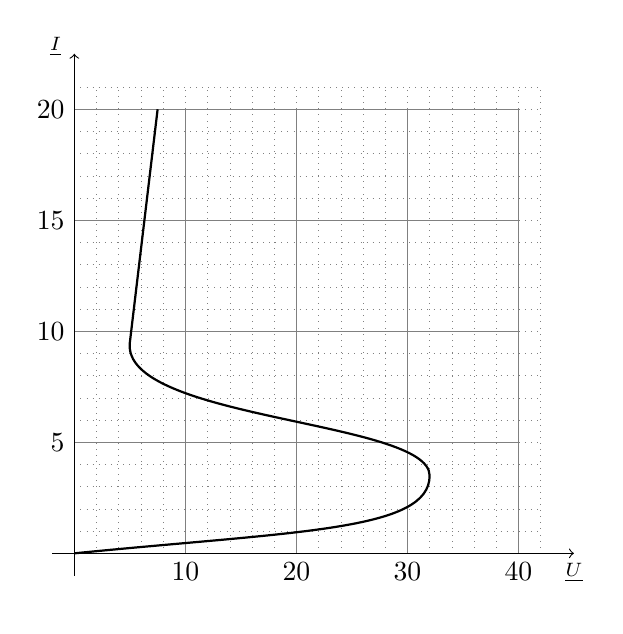
\begin{tikzpicture}[scale=1.41,
axes/.style=]

\draw[step=0.2, gray, dotted, very thin] (0,0) grid (4.2,4.2);
\draw[step=1, gray, very thin] (0,0) grid (4,4);

\begin{scope}[axes]
    \draw[->] (-0.2,0) -- (4.5,0) node[right, below] {$\frac{U}{\si{\volt}}$} coordinate(x axis);
    \draw[->] (0,-0.2) -- (0,4.5) node[above, left] {$\frac{I}{\si{\milli\ampere}}$} coordinate(y axis);

    \foreach \x/\xtext in {1/10, 2/20, 3/30, 4/40}
    \draw (\x,0) node[below] {$\xtext$};
    
    \foreach \y/\ytext in {1/5, 2/10, 3/15, 4/20}
    \draw (0,\y) node[left] {$\ytext$};
\end{scope}

\draw[thick] (0,0) .. controls (2,0.2) and (3.2,0.2) .. (3.2,0.7) .. controls (3.2,1.2) and (5/12,1.2) .. (0.5,1.9) -- (0.75,4);

\end{tikzpicture}

\end{center}
\end{figure}
\fi


\ifEngHint
According to the first law of Kirchhoff $V = U - IR$ must apply for a random voltage and current strength, $V$ is the voltage on the thyristor. Carrying the respective function to current-voltage characteristic you can see that for a certain voltage $U$ there are up to three solutions for $I$ and $V$, moreover a point with a negative slope is not stable because it would correspond to a negative resistance. With the given information it is possible to find how the current going through the thyristor changes when increasing the voltage of the voltage source.
\fi


\ifEngSolution
\begin{figure}[h]
\begin{center}
\begin{tikzpicture}[scale=1.4,
axes/.style=]

%\draw[step=0.2, gray, dotted, very thin] (0,0) grid (4,4);
\draw[step=1, gray, ultra thin] (0,0) grid (4,4);

\begin{scope}[axes]
    \draw[->] (-0.2,0) -- (4.5,0) node[below] {$\frac{V_1}{\si{\volt}}$} coordinate(x axis);
    \draw[->] (0,-0.2) -- (0,4.5) node[left] {$\frac{I}{\si{\milli\ampere}}$} coordinate(y axis);

    \foreach \x/\xtext in {1/10, 2/20, 3/30, 4/40}
    \draw (\x,0) node[below] {$\xtext$};
    
    \foreach \y/\ytext in {1/5, 2/10, 3/15, 4/20}
    \draw (0,\y) node[left] {$\ytext$};
\end{scope}

\draw [thick, name path=func] (0,0) .. controls (2,0.2) and (3.2,0.2) .. (3.2,0.7) .. controls (3.2,1.2) and (5/12,1.2) .. (0.5,1.9) -- (0.75,4);

\path
let
\n0 = {2.7}
in
coordinate (E0) at (\n0,0)
coordinate (W0) at (0,\n0);

\draw [dashed, thin, red, name path=example] (E0) -- (W0);

\fill [name intersections={of=func and example, by={a,b,c}}]
[red, opacity=0.5, every node/.style={above right, black, opacity=1}] (a) circle (1pt) node {\footnotesize $A$} (b) circle (1pt) node {\footnotesize $B$} (c) circle (1pt) node {\footnotesize $C$};

\path
let
\n1 = {3.96}
in
coordinate (E1) at (\n1,0)
coordinate (W1) at (0,\n1);

\draw [name path=line 1] (E1) -- (W1);

\fill [name intersections={of=func and line 1, by={a,c,b}}]
[red, opacity=0.5, every node/.style={below left, black, opacity=1}] (a) circle (1pt) node {\footnotesize $1$} (b) circle (1pt) node {\footnotesize $2$};

\path
let
\n2 = {4.2}
in
coordinate (E2) at (\n2,0)
coordinate (W2) at (0,\n2);

\draw [name path=line 2] (E2) -- (W2);

\fill [name intersections={of=func and line 2, by={a}}]
[red, opacity=0.5, every node/.style={above right, black, opacity=1}] (a) circle (1pt) node {\footnotesize $3$};

%\draw let \n1={0.815} in (0,\n1) -- (4,\n1);
%\draw let \n1={3.296} in (0,\n1) -- (4,\n1);
%\draw let \n1={3.509} in (0,\n1) -- (4,\n1);
\end{tikzpicture}
\end{center}
\end{figure}

Based on the Kirchhoff’s first law the relation $V_1 = U - IR$ must apply for a random voltage and current strength, where $V_1$ is the voltage on the thyristor $T_1$. Physically realistic situations are the ones where $V_1$ and $I$ are allowed by the thyristor’s I-V curve. In general there are up to three solutions for some voltage $U$ (the red line on the graph); the point $B$ is not stable because it would match a negative resistance and the points $A$ and $C$ are allowed but they match to different regimes which depend on how a point has been reached. Based on the aforementioned it is possible to sketch a graph for current strength. Initially the current strength increases approximately linearly because the thyristor behaves similarly to a linear resistor of resistance $r_1=\SI{20}{\kilo\ohm}$, which is why the initial slope of the current strength’s graph is $\frac{1}{R + r_1}=\frac{1}{\SI{22}{\kilo\ohm}}$. Near the point $1$ (voltage 39.6 V, current strength 4.1 mA) the current strength starts to increase rapidly and jumps to point $2$ (voltage 39.6 V, current strength 16.5 mA). Next the thyristor will again behave linearly with the resistance $r_2=\SI{0.24}{k\ohm}$ until the final point $3$ (voltage 42 V, current strength 17.5 mA). The current strength $I_a$ can be found more precisely by using the Kirchhoff’s laws and approximating the thyristor’s resistance linearly. Then we get $I_a = \SI{17.54}{\milli\ampere}$.

\begin{figure}[h]
\begin{center}
\begin{tikzpicture}[scale=1.4,
axes/.style=]

%\draw[step=0.2, gray, dotted, very thin] (0,0) grid (5,4);
\draw[step=1, gray, ultra thin] (0,0) grid (5,4);

\begin{scope}[axes]
    \draw[->] (-0.2,0) -- (5.5,0) node[below] {$\frac{t}{\si{\second}}$} coordinate(x axis);
    \draw[->] (0,-0.2) -- (0,4.5) node[left] {$\frac{I}{\si{\milli\ampere}}$} coordinate(y axis);

    \foreach \x/\xtext in {1/10, 2/20, 3/30, 4/40, 5/50}
    \draw (\x,0) node[below] {$\xtext$};
    
    \foreach \y/\ytext in {1/5, 2/10, 3/15, 4/20}
    \draw (0,\y) node[left] {$\ytext$};
\end{scope}

\draw let \n1={3.9615}, \n2={0.815} in [thick] (0,0) .. controls (2.2,0.2) and ($(\n1,0.3)-(0.1,0)$) .. (\n1,\n2);
\draw let \n1={3.9615}, \n2={0.815}, \n3={3.296} in [dashed] (\n1,\n2) -- (\n1,\n3);
\draw let \n1={3.9615}, \n2={0.815}, \n3={3.296}, \n4={3.509} in [thick] (\n1,\n3) -- (4.2,\n4);

\fill let \n1={3.9615}, \n2={0.815}, \n3={3.296}, \n4={3.509} in [red, opacity=0.5, thick, every node/.style={above left, black, opacity=1}] (\n1,\n2) circle (1pt) node {\footnotesize $1$} (\n1,\n3) circle (1pt) node {\footnotesize $2$} (4.2,\n4) circle (1pt) node {\footnotesize $3$};

\end{tikzpicture}
\end{center}
\end{figure}

After closing the switch we solve the current circuit based on the Kirchhoff’s laws. $U = IR + V_1 = IR + V_2$, $I = I_1 + I_2$, where $I_1^0=\SI{-11.5}{mA}$ is the y-intercept of the second linear part of the thyristor’s I-V curve. While solving we assume that $T_2$ is in a linear regime before a jump (similarly to the point $A$) and $T_1$ after a jump (similarly to the point $C$). We get that $I_1 = I_1^0 + \frac{V_1}{r_2}$ and $I_2 = V_2/r_1$. Solving this we get the voltages of the thyristors to be $V_1 = V_2$, current strength through the resistor $I = I_1^0 + V_1/r_1 + V_1/r_2$, voltages on the current source $U = I_1^0R + V_1R/r_2 + V_1R/r_1 + V_1$ and the voltages on the thyristors $V_1 = V_2 = \frac{U - I_1^0R}{R/r_1 + R/r_2 + 1} = \SI{6.84}{\volt}$. Therefore $I_1 = \SI{17.2}{\milli\ampere}$ and $I_2 = \SI{0.34}{\milli\ampere}$ that justifies the assumptions made.
\fi
}